%%%%%%%%%%%%%%%%%%%%%%%%%%%%%%%%%%%%%%%%%
% Classicthesis-Styled CV
% LaTeX Template
% Version 1.0 (22/2/13)
%
% This template has been downloaded from:
% http://www.LaTeXTemplates.com
%
% Original author:
% Alessandro Plasmati
%
% License:
% CC BY-NC-SA 3.0 (http://creativecommons.org/licenses/by-nc-sa/3.0/)
%
%%%%%%%%%%%%%%%%%%%%%%%%%%%%%%%%%%%%%%%%%

%----------------------------------------------------------------------------------------
%	PACKAGES AND OTHER DOCUMENT CONFIGURATIONS
%----------------------------------------------------------------------------------------

\documentclass{scrartcl}

\reversemarginpar % Move the margin to the left of the page 

\newcommand{\MarginText}[1]{\marginpar{\raggedleft\itshape\small#1}} % New command defining the margin text style

\usepackage[utf8]{inputenc}
%\usepackage[applemac]{inputenc}
\usepackage[nochapters]{classicthesis} % Use the classicthesis style for the style of the document
\usepackage[LabelsAligned]{currvita} % Use the currvita style for the layout of the document
\usepackage{graphicx}

\renewcommand{\cvheadingfont}{\LARGE\color{Maroon}} % Font color of your name at the top

\usepackage{hyperref} % Required for adding links	and customizing them
\hypersetup{colorlinks, breaklinks, urlcolor=Maroon, linkcolor=Maroon} % Set link colors

\newlength{\datebox}\settowidth{\datebox}{Set 2007-Ott 2010} % Set the width of the date box in each block

\newcommand{\NewEntry}[3]{\noindent\hangindent=2em\hangafter=0 \parbox{\datebox}{\small \textit{#1}}\hspace{1.0em} #2 #3 % Define a command for each new block - change spacing and font sizes here: #1 is the left margin, #2 is the italic date field and #3 is the position/employer/location field
\vspace{0.5em}} % Add some white space after each new entry

\newcommand{\Description}[1]{\hangindent=2em\hangafter=0\noindent\raggedright\footnotesize{#1}\par\normalsize\vspace{1em}} % Define a command for descriptions of each entry - change spacing and font sizes here

%----------------------------------------------------------------------------------------

\begin{document}

\thispagestyle{empty} % Stop the page count at the bottom of the first page

%----------------------------------------------------------------------------------------
%	NAME AND CONTACT INFORMATION SECTION
%----------------------------------------------------------------------------------------

\begin{cv}{\spacedallcaps{Matteo Facchini}}\vspace{1.5em} % Your name

\noindent\spacedlowsmallcaps{Informazioni Personali}\vspace{0.5em} % Personal information heading

\MarginText{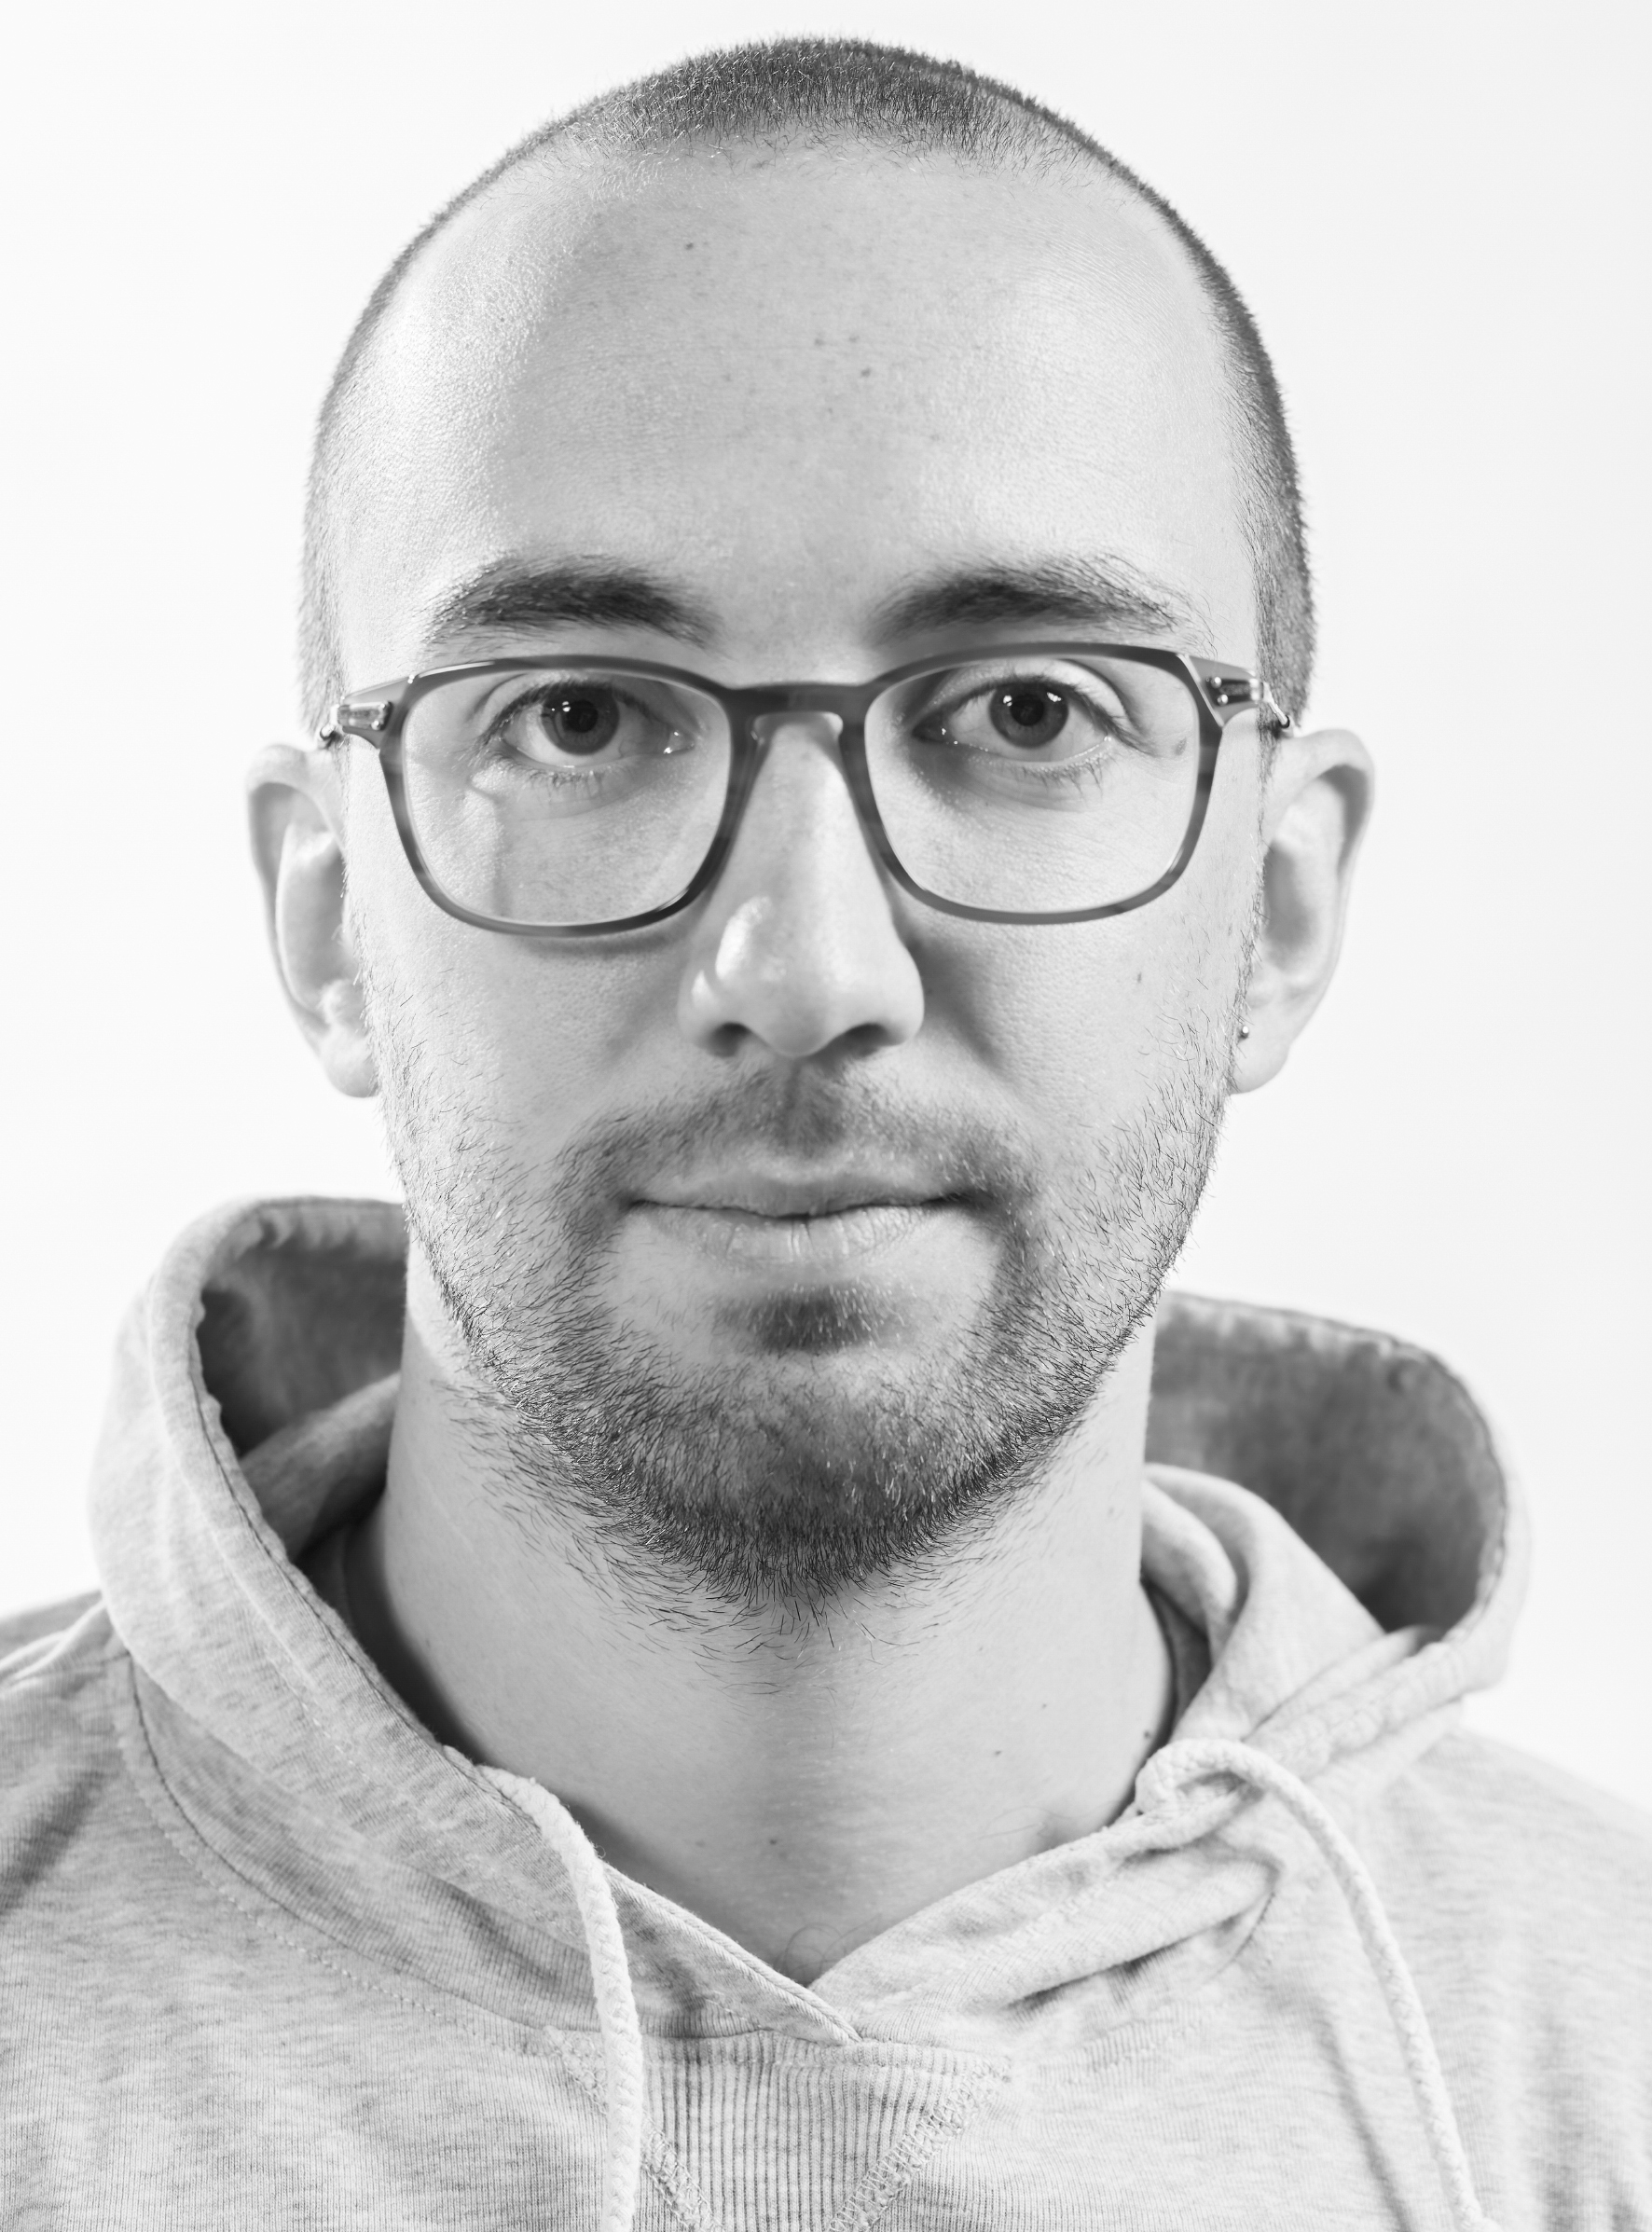
\includegraphics[width=3cm]{Facchini_Bild_2017_bw}}

\NewEntry{}{\textit{Nato a Trento (TN), Italia,}}{11 Febbraio 1988} % Birthplace and date

\NewEntry{}{cittadinanza italiana} % citizenship

\NewEntry{email}{\href{mailto:mat.facchini@gmail.com}{mat.facchini@gmail.com}} % Email address

%\NewEntry{pagina web}{\href{http://www.vaw.ethz.ch/en/people/person-detail.html?persid=203935}{http://www.vaw.ethz.ch/en/people/facchini}} % Personal website

% \NewEntry{LinkedIn}{\href{https://www.linkedin.com/in/matteo-facchini-1098a393}{https://www.linkedin.com/in/matteo-facchini}}

\NewEntry{telefono}{(U) +39 0461 236000 $\cdotp$\ \ (L) +39 338 490 1771} % Phone number(s)

\NewEntry{}{(C) +39 340 230 4434} % Phone number(s)

\vspace{1em} % Extra white space between the personal information section and goal
%
%\noindent\spacedlowsmallcaps{Goal}\vspace{1em} % Goal heading, could be used for a quotation or short profile instead
%
%\Description{Gain fundamental experience in my area of interest and expertise.}\vspace{2em} % Goal text


%----------------------------------------------------------------------------------------
%	EDUCATION
%----------------------------------------------------------------------------------------

\spacedlowsmallcaps{Educazione e Formazione}\vspace{1em}

\NewEntry{Gen 2020}{Ordine degli Ingegneri di Trento}

\Description{\MarginText{Iscrizione Albo}Iscrizione all'Albo degli Ingegneri Sez. A settore Civile e Ambientale, della provincia di Trento, al n. 4371 dal 20/01/2020, ai sensi del D.P.R. 328 / 2001.}

%------------------------------------------------

\NewEntry{Dic 2019}{Seconda sessione dell'anno 2019}

\Description{\MarginText{Esame di Stato}Esame di stato per l'abilitazione alla professione di ingegnere, Universit\`a degli Studi di Trento -- Trento (TN), Italia}

%------------------------------------------------

\NewEntry{Nov 2013-Gen 2018}{ETH Zurich -- Zurigo, Svizzera}

\Description{\MarginText{Dottorato}Versuchsanstalt f\"ur Wasserbau, Hydrologie und Glaziologie (VAW)\newline 
	Tesi: \textit{Downstream morphological effects of Sediment Bypass Tunnels}\newline 
	Descrizione: monitoraggio e modellazione degli effetti dei rilasci di acqua e sedimenti da un tunnel-bypass (SBT) sul tratto di fiume a valle del tunnel.\newline
	Supervisori: Prof.~Robert M. \textsc{Boes} \& Dr.~Annunziato \textsc{Siviglia}}

%------------------------------------------------

\NewEntry{Ott 2010-Nov 2013}{Universit\`a degli Studi di Trento -- Trento (TN), Italia}

\Description{\MarginText{Laurea Magistrale}Ingegneria per l'Ambiente e il Territorio\newline 
Tesi: \textit{High order ADER-WENO finite volume schemes for Boussinesq-type equations} (votazione 104/110)\newline
Relatore: Prof.~Michael \textsc{Dumbser}}

%------------------------------------------------

\NewEntry{Set 2011-Set 2012}{Technische Univerit\"at Dresden -- Dresda, Germania}

\Description{\MarginText{Erasmus}Ingegneria Civile ed Ambientale\newline}

%------------------------------------------------

\NewEntry{Set 2007-Ott 2010}{Universit\`a degli Studi di Trento -- Trento (TN), Italia}

\Description{\MarginText{Laurea Triennale}Ingegneria Ambientale\newline
Tesi: \textit{Aspetti dei deflussi di pioggia: dilavamento di superfici stradali e rischi per i bacini limitrofi} (votazione 99/110)\newline
Relatori: Prof.~Sandra \textsc{Dirè} \& Prof.~Maurizio \textsc{Righetti}}

%------------------------------------------------
%
%\NewEntry{Set 2002-Lug 2007}{Liceo Scientifico Statale “G. Galilei” -- Trento (TN), Italia}
%
%\Description{\MarginText{Maturit\`a}Liceo Scientifico, Corso P.N.I. (Piano Nazionale Informatico) \newline
%Diploma di scuola superiore, maturit\`a scientifica (votazione 84/100)}

%------------------------------------------------

% \vspace{1em} % Extra space between major sections
\newpage
%----------------------------------------------------------------------------------------
%	WORK EXPERIENCE
%----------------------------------------------------------------------------------------

\noindent\spacedlowsmallcaps{Esperienza Lavorativa}\vspace{1em}

\NewEntry{Mar 2022-presente}{Funzionario Tecnico - Ingegnere, \textsc{Autorità di Bacino Distrettuale delle Alpi Orientali} -- Trento, Italia}

\Description{\MarginText{AdBDAO}Modellazione di fenomeni di alluvione torrentizia e colata detritica per la mappatura del pericolo in aree soggette a rischio idrogeologico.}

\Description{Componente della commissione giudicatrice della gara a procedura aperta per l'affidamento del servizio di riqualificazione fluviale del tratto terminale del fiume Piave - attivazione di campagne di informazione e comunicazione finalizzate al coinvolgimento dei cittadini nel monitoraggio ambientale (CIG 9456138BED).}

\Description{Componente della commissione giudicatrice della gara a procedura aperta per l'affidamento del servizio di realizzazione di due cortometraggi per la divulgazione del progetto denominato "osservatorio dei cittadini sulle acque" (CIG 9669978E46).}

\Description{Direttore per l'Esecuzione del Contratto per l'appalto relativo al servizio di "Riqualificazione Fluviale del tratto terminale del Fiume Piave - Misure in alveo di portata in diverse condizioni idrologiche e installazione sensori" (CIG 7887115D2F).}

%------------------------------------------------

\NewEntry{Giu 2023}{Formatore, \textsc{Ordine dei Geologi e Ordine degli Ingegneri della Regione Autonoma Friuli-Venezia Giulia} -- Pordenone (PN), Italia}

\Description{\MarginText{OdG-OdI FVG}Attività formativa riguardante la modellazione morfodinamica di corsi d'acqua con l'utilizzo di BASEMENT per casi reali.}

%------------------------------------------------

\NewEntry{Feb 2022}{Formatore, \textsc{Zollet Ingegneria srl} -- Santa Giustina (BL), Italia}

\Description{\MarginText{Zollet}Attività formativa riguardante la modellazione morfodinamica di corsi d'acqua con l'utilizzo di BASEMENT per casi reali.}

%------------------------------------------------

\NewEntry{Mag 2019-Gen 2022}{Funzionario Tecnico - Ingegnere, \textsc{Autorità di Bacino Distrettuale delle Alpi Orientali} -- Trento, Italia}

\Description{\MarginText{AdBDAO}Modellazione di fenomeni di alluvione torrentizia e colata detritica per la mappatura del pericolo in aree soggette a rischio idrogeologico.}

%------------------------------------------------

\NewEntry{Feb 2019-Apr 2019}{Formatore, \textsc{Studio API} -- Feltre, Italia}

\Description{\MarginText{Studio API}Attività formativa riguardante la modellazione morfodinamica di corsi d'acqua con l'utilizzo di BASEMENT per casi reali.}

%------------------------------------------------

\NewEntry{Mag 2018-Mag 2019}{Assegnista di ricerca, \textsc{Università degli Studi di Trento} -- Trento, Italia}

\Description{\MarginText{UniTN}Modellazione degli effetti di rilasci di sedimenti ripetuti in fiumi alimentati da ghiacciaio.}

%------------------------------------------------

\NewEntry{Nov 2013-Gen 2018}{Dottorando, \textsc{ETH Zurich} -- Zurigo, Svizzera}

\Description{\MarginText{ETH Zurich}Monitoraggio e modellazione degli effetti dei rilasci di acqua e sedimenti da un tunnel-bypass (SBT) sul tratto di fiume a valle del tunnel.}

%------------------------------------------------

\NewEntry{Nov 2013-Ott 2017}{Sviluppatore, \textsc{ETH Zurich} -- Zurigo, Svizzera}

\Description{\MarginText{ETH Zurich}Sviluppatore del software BASEMENT (Basic Simulation Environment for Computation of Environmental Flow and Natural Hazard Simulation), usato nell'ambito dell'ingegneria fluviale e della modellazione morfodinamica.}

%------------------------------------------------

% \NewEntry{Gen-Mar 2013}{Tutor, \textsc{LEONARDO Formazione e Sviluppo} -- Catania (CT), Italia}

% \Description{\MarginText{LEONARDO}Tutoraggio a studenti di vari licei del Trentino che hanno parteciato ad una simulazione del funzionamento delle Nazioni Unite (National Model United Nations, NMUN) a New York, USA.}

%------------------------------------------------
%
%\NewEntry{Set 2010-Ago 2011}{Tecnico Suono e Luci, \textsc{Opera Universitaria} -- Trento (TN), Italia}
%
%\Description{\MarginText{Op. Univ. TN}Tecnico suono e luci e aiuto palco presso l'ufficio cultura dell'Opera Universitaria di Trento.}
%
%%------------------------------------------------
%
%\NewEntry{2005-2007}{Impiegato a progetto, \textsc{Istituto Comprensivo Trento 3} -- Trento (TN), Italia}
%
%\Description{\MarginText{Ist. Comp. TN3}Implementazione dei dati relativi ai questionari di autovalutazione dell'istituto.}
%
%------------------------------------------------

\vspace{1em} % Extra space between major sections

% %----------------------------------------------------------------------------------------
% %	PUBLICATIONS
% %----------------------------------------------------------------------------------------

% \spacedlowsmallcaps{Pubblicazioni accademiche}\vspace{1em}

% \Description{\MarginText{2022}
% 	M. \textsc{Facchini}, (2018), Downstream morphological effects of Sediment Bypass Tunnels, VAW Mitteilungen 243 (R.M. Boes ed.), ETH Z\"urich, Svizzera.}

% %------------------------------------------------

% \Description{\MarginText{2019}
% 	M. \textsc{Facchini}, ~R.M. \textsc{Boes}, ~D.F. \textsc{Vetsch}, ~A.\textsc{Siviglia} (2018), Riverbed and surface composition adjustments in a gravel-bed river subject to repeated Sediment Bypass Tunnel operations, in revisione}

% %------------------------------------------------

% \Description{\MarginText{2017}
% 	M. \textsc{Facchini}, ~A. \textsc{Siviglia}, ~R. M. \textsc{Boes}, (2017), Downstream morphological effects of SBT releases: 1D numerical study and preliminary LiDAR data analysis, In: Proceedings of the 2$^{nd}$ International Workshop on Sediment Bypass Tunnels (T. Sumi ed.), Kyoto University, Kyoto, Japan.}

% 	\Description{
% 	M. \textsc{Döring}, ~M. \textsc{Facchini}, ~S. \textsc{Fink}, ~M. J.\textsc{Franca}, ~E. \textsc{Martín Sanz}, ~Ch. \textsc{Robinson}, ~Ch. \textsc{Scheidegger}, ~A. \textsc{Siviglia}, ~C. \textsc{Trautwein}, ~D. \textsc{Vetsch}, ~Ch. \textsc{Weber}, (2017), Dinamica dei sedimenti e misurazione dei suoi effetti. In: Dinamica dei sedimenti e degli habitat. Ufficio federale dell’ambiente (UFAM), Berna. Scheda 2.}

% 	\Description{
% 	M. \textsc{Facchini}, ~E. \textsc{Martín Sanz}, ~S. \textsc{Fink}, ~D. \textsc{Vetsch}, ~Ch. \textsc{Robinson}, ~M. \textsc{Döring}, ~A. \textsc{Siviglia}, ~Ch. \textsc{Scheidegger}, ~R. M. \textsc{Boes}, (2017), Gallerie bypass dei sedimenti e piene artificiali. In: Dinamica dei sedimenti e degli habitat. Ufficio federale dell’ambiente (UFAM), Berna. Scheda 6.}

% %------------------------------------------------

% \Description{\MarginText{2016}
% 	M. \textsc{Dumbser}, ~M. \textsc{Facchini}, (2016), A space-time discontinuous Galerkin method for Boussinesq- type equations, Applied Mathematics and Computation, 272(2): 336-346.}

% %------------------------------------------------

% \Description{\MarginText{2015}
% 	M. \textsc{Facchini}, ~A. \textsc{Siviglia}, ~R. M. \textsc{Boes}, (2015), Downstream morphological impact of a sediment bypass tunnel -- preliminary results and forthcoming actions, In: Proc. First International Workshop on Sediment Bypass Tunnels, VAW Mitteilungen 232, ETH Z\"urich, Schweiz, 137-146.}

% %------------------------------------------------

% \vspace{1em} % Extra space between major sections

%----------------------------------------------------------------------------------------
%	CONFERENCES AND COURSES
%----------------------------------------------------------------------------------------
\newpage
\spacedlowsmallcaps{Formazione post universitaria:}\vspace{1em}

\Description{\MarginText{2023}FAD - GIS Open Source Avanzato (QGIS) -- Trento, Italia -- marzo 2023.}

\Description{\MarginText{}World Landslide Forum 2023 -- Firenze, Italia -- novembre 2023.}

\Description{\MarginText{}FAD - CStatistica di base (2 ore - 2 CFP) - Formazione per Ingegneri -- online -- novembre 2023.}

\Description{\MarginText{}FAD - Consulente tecnico d'ufficio - c.t.u. (12 ore - 12 CFP) - Formazione per Ingegneri -- online -- novembre 2023.}

\Description{\MarginText{2022}FAD - La responsabilità professionale del tecnico -- Trento, Italia -- novembre 2022.}

\Description{\MarginText{}FAD - Coordinare le coordinate: datum planimetrici ed altimetrici -- Trento, Italia -- novembre 2022.}

\Description{\MarginText{2021}FAD - Corso di etica e deontologia -- Trento, Italia -- dicembre 2021.}

\Description{\MarginText{2019}Corso di formazione sull'utilizzo di HEC-RAS -- Trento, Italia -- maggio-giugno 2019.}

\Description{\MarginText{}Corso di formazione sulla modellazione dei fenomeni di colata detritica -- Trento, Italia -- settembre-ottobre 2019.}

\Description{\MarginText{2018}American Geophysical Union (AGU) Fall Meeting -- Washington DC, USA -- 11-15 dicembre 2018.}

\Description{\MarginText{}Seminario al St. Anthony Falls Laboratory -- Minneapolis, USA -- 4 dicembre 2018.}

\Description{\MarginText{2017}Second International Workshop on Sediment Bypass Tunnels -- Kyoto, Giappone -- 9-12 maggio 2017.}

\Description{\MarginText{2016}Summer School on Fluvial Geomorphology -- Losone, Svizzera -- 27 giugno - 1 luglio 2016.}

\Description{\MarginText{2015}Introduction to Writing at Doctoral Level, Natural Science \& Engineering, C1 level -- Zurigo, Svizzera -- febbraio-maggio 2015.}

\Description{\MarginText{}First International Workshop on Sediment Bypass Tunnels -- Zurigo, Svizzera -- 27-29 aprile 2015.}

\Description{\MarginText{2014}European Geoscience Union (EGU) General Assembly -- Vienna, Austria -- 27 aprile - 2 maggio 2014.}

\Description{\MarginText{}Post-graduate Course on Advanced Numerical Methods for Hyperbolic Equations and Applications -- Trento (TN), Italia -- 3-14 febbraio 2014.}

\Description{\MarginText{}Post-graduate Course on Basic Interdisciplinary River Morphodynamics: First Edition, River Bars -- Trento (TN), Italia -- 27-31 ottobre 2014.}

%------------------------------------------------

\vspace{4em} % Extra space between major sections
% \newpage
%----------------------------------------------------------------------------------------
%	PERSONAL SKILLS
%----------------------------------------------------------------------------------------
\newpage
\spacedlowsmallcaps{Competenze linguistiche}\vspace{1em}

\vspace{1em}

\newlength{\langbox} % Create a new length for the length of languages to keep them equally spaced
\settowidth{\langbox}{English} % Length equals the length of "English" - if you have a longer language in your list put it here

\Description{\MarginText{Madrelingua}\parbox{\langbox}{\textsc{Italiano}}}

\vspace{-0.5em} % Negative vertical space to counteract the vertical space between every \Description command

\Description{\MarginText{Altre lingue}\parbox{\langbox}{\textsc{Inglese}}\vspace{0.2em}
	\begin{tabular}{ c c c c c }
		\multicolumn{2}{c}{COMPRENSIONE} & \multicolumn{2}{c}{PARLATO} & SCRITTO \\
		Ascolto & Lettura & Interazione orale & Produzione orale &  \\
		C1 & C1 & C1 & C1 & C1 \\
	\end{tabular}
}
\Description{\parbox{\langbox}{\textsc{Tedesco}}\vspace{0.2em}	
	\begin{tabular}{ c c c c c }
		\multicolumn{2}{c}{COMPRENSIONE} & \multicolumn{2}{c}{PARLATO} & SCRITTO \\
		Ascolto & Lettura & Interazione orale & Produzione orale &  \\
		C1 & C1 & C1 & C1 & C1 \\
		\multicolumn{5}{c}{Patentino bilinguismo A}
	\end{tabular}
}

% %----------------------------------------------------------------------------------------
% %	TECHINICAL SKILLS
% %----------------------------------------------------------------------------------------

% \spacedlowsmallcaps{Capacit\`a e competenze tecniche}\vspace{1em}

% \vspace{1em}

% \Description{\MarginText{Monitoraggio fluviale diretto}Ottima esperienza: raccolta dati in ambiente GIS con tecniche di mobile mapping, misure di granulometria, velocità di deflusso, topografia, ecc.}
	
% \Description{\MarginText{Monitoraggio fluviale indiretto}Ottima esperienza: fotogrammetria aerea e scansioni 3D mediante Laser Imaging Detection and Ranging (LiDAR).}

% \Description{\MarginText{mesoHABSIM}Buona conoscenza: valutazione e modellazione dell’habitat di ambienti fluviali e torrentizi (metodologia mesoHABSIM per la classificazione delle unità morfologiche fluviali).}

% \Description{\MarginText{Ambienti informatici}Macintosh, Windows e Ubuntu e relative funzionalità di base (p.e. pacchetti office, iWork e LibreOffice).}

% \Description{\MarginText{Gestione Server}Gestione, organizzazione ed utilizzo server sia Ubuntu che Windows.}

% \Description{\MarginText{Programmazione e Scripting}Ottima conoscenza: Python, Matlab, R e GitHub. 
	
% Buona conoscenza: C++ e Fortran.}

% \Description{\MarginText{BASEMENT}Ottima conoscenza: ingegneria fluviale e modellazione morfodinamica (sviluppato presso VAW (ETH Zurich)).}

% \Description{\MarginText{HEC-RAS}Ottima conoscenza: ingegneria fluviale e modellazione morfodinamica (sviluppato presso Hydrologic Engineering Center - US Army Corps of Engineers).}

% \Description{\MarginText{QGIS}Ottima conoscenza: applicazioni nell'ambito della valutazione dell'evoluzione topografica di fiumi, ovvero valutazione delle modifiche dei modelli digitali di elevazione (DEM).}

% \Description{\MarginText{GCD}Ottima conoscenza: valutazione delle modifiche dei modelli digitali di elevazione (DEM) con valutazione statistica degli errori di calcolo.}

% \Description{\MarginText{LaTeX}Ottima conoscenza: scrittura di testi e report.}

% \Description{\MarginText{HydroVISH}Ottima conoscenza: classificazione dei punti misurati con laser scanner durante voli LiDAR (sviluppato da AHM (Innsbruck)).}

% \Description{\MarginText{Altri Software}Conoscenza sufficiente: Docker, Maple, Ansys CFX e Comsol Multiphysics.}

% \vspace{1em} % Extra space between major sections

% %----------------------------------------------------------------------------------------
% %	GENERAL SKILLS
% %----------------------------------------------------------------------------------------

% \spacedlowsmallcaps{Capacit\`a e competenze generali}\vspace{1em}

% \vspace{1em}

% %\newlength{\langbox} % Create a new length for the length of languages to keep them equally spaced
% %\settowidth{\langbox}{Italiano} % Length equals the length of "English" - if you have a longer language in your list put it here
% %
% %\Description{\MarginText{Lingue}\parbox{\langbox}{\textsc{Italiano}}\ \ $\cdotp$\ \ \ Madrelingua}
% %
% %\vspace{-0.5em} % Negative vertical space to counteract the vertical space between every \Description command
% %
% %\Description{\parbox{\langbox}{\textsc{Inglese}}\ \ $\cdotp$\ \ \ Fluente -- livello C1}
% %
% %\vspace{-0.5em} % Negative vertical space to counteract the vertical space between every \Description command
% %
% %\Description{\parbox{\langbox}{\textsc{Tedesco}}\ \ $\cdotp$\ \ \ Fluente -- livello C1}

% \Description{\MarginText{Capacit\`a e competenze relazionali}capacità di parlare in pubblico.
% \vspace{0.5em}
% \newline
% abilità didattiche.
% \vspace{0.5em}
% \newline
% attitudine a lavorare in gruppo.
% \vspace{0.5em}
% \newline
% orientamento a farsi carico delle responsabilit\`a.}

% \Description{\MarginText{Capacit\`a e competenze organizzative}capacit\`a di gestire pi\`u attivit\`a contemporaneamente.
% \vspace{0.5em}
% \newline
% esperienza in organizzazione di eventi pubblici di media affluenza (concerti dell'orchestra "I Filarmonici" di Trento e del Corpo musicale Citt\`a di Trento; ballo in maschera del Corpo Musicale Citt\`a di Trento).}

% \Description{\MarginText{Capacit\`a e competenze artistiche}\parbox{\langbox}{\textsc{Musica}}\ \ $\cdotp$\ \ \ diploma della scuola di musica "I Minipolifonici" di Trento in percussioni; svariati anni di attivit\`a concertistica con l'orchestra "I Filarmonici" di Trento (musica classica), con le orchestre TU-Sinfonieorchester e TU-Kammerphilharmonie dell'Universit\`a Tecnica di Dresda (musica classica), con il Corpo Musicale Citt\`a di Trento (musica classica e popolare) e in formazioni locali (musica leggera).}

% \Description{\MarginText{Altre capacit\`a e competenze}membro del direttivo dell'orchestra "I Filarmonici" di Trento fino al 2013.
% \vspace{0.5em}
% \newline
% membro del direttivo del Corpo Musicale Citt\`a di Trento fino al 2013.
% \vspace{0.5em}
% \newline
% membro del comitato artistico del Corpo Musicale Citt\`a di Trento fino al 2013.
% \vspace{0.5em}
% \newline
% rappresentante degli studenti del Liceo Scientifico Statale "G. Galilei" di Trento durante gli anni scolastici 2005-2006 e 2006-2007.
% \vspace{0.5em}
% \newline
% rappresentante degli studenti nel Consiglio di Facoltà della Facoltà di Ingegneria dell'Università degli Studi di Trento durante l'anno accademico 2010-2011.}

% \Description{\MarginText{Patente} Patenti B (mezzo proprio) ed A.}

% \vspace{1em} % Negative vertical space to counteract the vertical space between every \Description command

%------------------------------------------------

%\Description{\MarginText{Interests}Percussions\ \ $\cdotp$\ \ Music\ \ $\cdotp$\ \ Sports\ \ $\cdotp$\ \ Reading\ \ $\cdotp$\ \ Movies}

%----------------------------------------------------------------------------------------

\date{Trento, 17 gennaio 2024}

\end{cv}

\end{document}